%Template pembuatan proposal skripsi.
\documentclass{jtetiproposalskripsi}
\usepackage{url}

%-----------------------------------------------------------------
%Disini awal masukan untuk data proposal skripsi
%-----------------------------------------------------------------
\titleind{ANALISA DAN PERANCANGAN WEB SERVICE UJIAN ONLINE BERBASIS SOAP (STUDI KASUS PADA ELEARNING UNIVERSITAS MUHAMMADIYAH JEMBER)}

\fullname{MOHAMMAD SYAHRONI}

\idnum{11/1065/TI/1045}

\approvaldate{08 januari 2015}

\degree{Sarjana Teknik Informatika}

\yearsubmit{2015}

\program{Teknik Informatika}

\headprogram{Eko fajar S.T., M.T.}

\dept{Teknologi Informasi}

\firstsupervisor{Eko Fajar Y.,S.Kom}
\firstnip{1976 0501 2002 12 1 002}

\secondsupervisor{Triawan Adi Cahyanto}
\secondnip{1977 0131 2002 12 1 003}


%-----------------------------------------------------------------
%Disini akhir masukan untuk data proposal skripsi
%-----------------------------------------------------------------

\begin{document}

\cover

\approvalpage

%-----------------------------------------------------------------
%Disini akhir masukan untuk muka skripsi
%-----------------------------------------------------------------

%-----------------------------------------------------------------
%Disini awal masukan Intisari
%-----------------------------------------------------------------
\begin{abstractind}
Ujian online saat ini sudah tidak lagi menjadi trend di masyarakat karena teknologi yang ada pun semakin canggih. Platform yang ada semakin bermacam-macam sehingga  dengan adanya web service, aplikasi yang ada dapat digunakan pada lintas platform.  Web service merupakan software system yang dirancang untuk mendukung interopabilitas mesin ke mesin yang dapat berinteraksi melalui jaringan. Dengan begitu ujian online dapat dilaksanakan meskipun melalui handphone, PDA dll.


\bigskip
\textbf{Kata kunci} : \emph{web service}, \emph{platform}, ujian online.
\end{abstractind}
%-----------------------------------------------------------------
%Disini akhir masukan Intisari
%-----------------------------------------------------------------

\tableofcontents
\addcontentsline{toc}{chapter}{DAFTAR ISI}
\selectlanguage{bahasa}\clearpage\pagenumbering{arabic}\setcounter{page}{1}

%-----------------------------------------------------------------
%Disini awal masukan untuk Bab
%-----------------------------------------------------------------
\chapter{LATAR BELAKANG}

\section{Latar Belakang Masalah}
Dengan semakin besar dan kompleksnya suatu aplikasi maka pengelolaan dan integrasi menjadi hal yang sangat diperlukan.  \emph{Extensible Markup Language}(XML)web service memungkinkan suatu aplikasi dari berbagai platform bisa berhubungan satu sama lainnya. Sesuai dengan namanya, XML webservice tersimpan dalam suatu format .XML dimana dapat digunakan oleh aplikasi lain tanpa harus mengetahui detil dari pemrograman yang terdapat didalamnya. Sehingga hanya dengan XML web service satu model dapat diakses dan dipergunakan oleh bermacam-macam aplikasi dan device.

Universitas merupakan system yang kompleks dimana terdiri dari beberapa fakultas, jurusan dan bagian-bagian yang lain. Karena lingkup universitas lebih besar maka penerapan sistem informasi terpusat akan terlalu membebani server.  Sedangkan jika beberapa dari fakultas dalam universitas menggunakan platform yang berbeda-beda akan mengalami masalah ketika integrasi data dan fungsi yang berada pada platform berbeda-beda tersebut. Disamping itu juga apabila pengguna lebih cenderung pada device yang berbeda seperti handphone, PDA sehingga rancangan sistem informasi universitas akan semakin kompleks.

Penelitian ini dimakksudkan untuk menerapkan konsep XML websevice dengan kemempuan yang telah diuraikan sehingga dapat menjembatani beberapa aplikasi yang beda platform sehingga dapat terintegrasi dan terpusat. Adapun metode pengembangan sistem menggunakan metode waterfall dimana terdapat tahapan-tahapan yaitu analisa dan rekayasa system, analisis persyaratan, perancangan, coding, pengujian dan pemeliharaan.



\section{Rumusan Masalah}
\vspace{-0.5cm}

\begin{enumerate}[a.]
\begin{singlespace}
\itemsep0em
\item Bagaimana menjembatani beberapa sistem informasi pembelajaran dengan menggunakan teknologi webservice?
\item Bagaimana mendistribusikan informasi secara cepat dan akurat?
\end{singlespace}
\end{enumerate}

\section{Batasan Masalah}
\vspace{-0.5cm}

\begin{enumerate}[a.]
\begin{singlespace}
\itemsep0em
\item Layanan web service menggunakan XML berbasis SOAP pada sistem ujian online melalui web service.
\item Pengembangan layanan Elearning unmuh jember untuk meningkatkan mutu pendidikan di universitas muhammadiyah jember.
\end{singlespace}
\end{enumerate}

\section{Tujuan Penelitian}
Mempermudah mahasiswa universitas muhammadiyah dalam ujian online sehingga ujian dapat menggunakan media handphone, PDA, dll.

\section{Manfaat Penelitian}
Sebagai sistem ujian online yang dapat diakses melalui media/ device dengan platform yang berbeda-beda sehingga dapat mengurangi kinerja server.

%-------------------------------------------------------------------------------
\chapter{DASAR TEORI}                
\section{Landasan Teori}
\subsection{\emph{Web Service}}
Web service adalah sebuah software  yang dirancang untuk mendukung interoperabilitas interaksi mesin-ke-mesin melalui sebuah jaringan [1].  Web service  secara teknis memiliki mekanisme interaksi antar sistem sebagai penunjang interoperabilitas, baik berupa agregasi (pengumpulan) maupun sindikasi (penyatuan).  Web service  memiliki layanan terbuka untuk kepentingan integrasi data dan kolaborasi informasi yang bisa diakses melalui internet oleh berbagai pihak menggunakan teknologi yang dimiliki oleh masing-masing pengguna. Sekalipun mirip dengan Application Programming Interface  (API) berbasis web,  web service lebih unggul karena dapat dipanggil dari jarak jauh melalui internet. Pemanggilan web service  bisa menggunakan bahasa pemrograman apa saja dan dalam  platform apa saja, sementara API hanya bisa digunakan dalam  platform tertentu  [2].  

Web service dapat dipahami sebagai Remote Procedure Call  (RPC) yang mampu memproses fungsi-fungsi yang didefinisikan pada sebuah aplikasi  web dan mengekspos sebuah API atau  User Interface (UI) melalui web. 
\\
\\
Kelebihan web service  adalah:
\vspace{-0.5cm}
\begin{enumerate}[a.]
\begin{singlespace}
\itemsep0em
\item lintas  platform,
\item language independent,
\item jembatan penghubung dengan database  tanpa perlu  driver database dan tidak harus mengetahui jenis DBMS,
\item mempermudah proses pertukaran data, serta
\item penggunaan kembali komponen aplikasi  [2].
\end{singlespace}
\end{enumerate} 

Berdasarkan konsep hubungan dan penyampaian informasi, web service  dikembangkan melalui empat model arsitektur, masing-masing berorientasi pada  message,  action,  resource , dan policy. Pengembangan model yang diturunkan berdasarkan orientasi pada action (Service Oriented Model/SOM) menghasilkan  Services Oriented Architecture  (SOA), yaitu model arsitektur berbasis layanan. Sementara pengembangan model yang diturunkan berdasarkan orientasi pada  resource  ( Resource Oriented Model/ROM) menghasilkan Resource Oriented Architecture (ROA), yaitu model arsitektur berbasis sumberdaya informasi  [3].  

Dalam perkembangannya, model  web service  memiliki dua metode yang berorientasi pada layanan dan sumberdaya informasi, yaitu: SOAP (Simple Object Access Protocol ) dan REST ( REpresentational State Transfer). Impementasi model SOA telah banyak dilakukan dan dikembangkan oleh banyak  vendor  (misal: Microsoft, Sun dan IBM, melalui dukungan platform infrastruktur  .Net  dan Java).
\\
Proses layanan dengan arsitektur SOAP memiliki tiga komponen utama, yaitu:
\vspace{-0.5cm}
\begin{enumerate}[a.]
\begin{singlespace}
\itemsep0em
\item service provider ,
\item service requester , dan 
\item service broker , 
\end{singlespace}
\end{enumerate}
serta komponen pendukung yaitu: 
\vspace{-0.5cm}
\begin{enumerate}[a.]
\begin{singlespace}
\itemsep0em
\item XML,
\item SOAP-XML (terdiri atas  header  dan body ),
\item WSDL, serta 
\item UDDI  [4]. 
\end{singlespace}
\end{enumerate}
Metode REST telah dikembangkankan oleh  Fielding [5] yang didasari oleh empat prinsip utama teknologi, yaitu: 
\vspace{-0.5cm}
\begin{enumerate}[a.]
\begin{singlespace}
\itemsep0em
\item Resource identifier through Uniform Resource Identifier  (URI), 
\item Uniform interface (sumberdaya CRUD menggunakan operasi PUT, GET, POST, dan DELETE),
\item Self-descriptive messages (sumberdaya tidak terikat sehingga dapat mengakses konten HTML, XML, PDF, JPEG, plain text, meta data, dll), serta
\item Stateful interactions through hyperlinks  (bersifat  stateless)  [6].
\end{singlespace}
\end{enumerate}

Metode REST lebih sederhana karena menggunakan format standar (HTTP, HTML, XML, URI, MIME), namun jika diperlukan proses pertukaran data, maka konten berupa teks dari hasil eksekusi  web service  dapat diolah dalam format teks (seperti XML atau HTML) dengan menggunakan utilitas komunikasi data berupa koneksi  socket  protokol HTTP. Utilitas ini umumnya tersedia dalam pustaka komunikasi pada bahasa pemrograman (seperti Java, Visual Basic, Delphi, PHP, ASP, dan JSP) [3].


\subsection{XML (Extensible Markup Language)}
Menurut Walsh (1998), XML merupakan   sebuah Markup Language untuk dokumentasi terstruktur. Dokumen-dokumen terstruktur adalah dokumen-dokumen yang mempunyai isi/content (kata, gambar) serta indikasi yang menyatakan makna dari content tersebut.
XML mempunyai kelebihan sebagai berikut (Tidwell, 1999): 
\vspace{-0.5cm}
\begin{enumerate}[a.]
\begin{singlespace}
\itemsep0em
\item XML tidak tergantung pada platform atau system operasi yang digunakan. 
\item Hasil pencarian data lebih akurat. 
\item Dokumen XML dapat diterjemahkan ke dalam beberapa format yang berbeda karena dalam XML data dan instruksi dipisahkan.
\end{singlespace}
\end{enumerate}
 
Ada 6 jenis markup yang bisa muncul dalam sebuah dokumen XML yaitu:
\vspace{-0.5cm}
\begin{enumerate}[a.]
\begin{singlespace}
\itemsep0em
\item Elemen dan atribut. Elemen menyatakan sifat dari content yang dilingkupinya sedangkan atribut merupakan pasangan dari nama-nilai yang muncul dalam tag setelah  nama elemen. 
\item Entity reference, digunakan supaya tanda markup dapat dimasukkan ke dalam dokumen XML dan dianggap sebagai content. 
\item Comment atau komentar.
\item Processing Instruction (PI), memungkinkan dokumen berisi suatu instruksi untuk suatu aplikasi. 
\item CDATA Section. Dalam sebuah dokumen, CDATA Section menginstruksikan parser untuk mengabaikan karakter-karakter tertentu yang mungkin akan dikenali sebagai karakter markup.CDATA Section. Dalam sebuah dokumen, CDATA Section menginstruksikan parser untuk mengabaikan karakter-karakter tertentu yang mungkin akan dikenali sebagai karakter markup. 
\item Document  Type  Declaration  (DTD).  DTD  berisi  deklarasi  markup  yang  memenuhi  grammar  untuk  suatu    kelas dokumen.
\end{singlespace}
\end{enumerate}

XML Web Services dibangun berdasarkan teknologi yang terbuka seperti: 
\vspace{-0.5cm}
\begin{enumerate}[a.]
\begin{singlespace}
\itemsep0em
\item eXtensible Markup Language (XML).
\item Simple Object Access Protocol  (SOAP). 
\item Universal Description, Discovery and Integration (UDDI).
\item Web Servicess Description Language (WSDL).
\end{singlespace}
\end{enumerate}

\subsection{SOAP (Simple Object Access Protocol)}
SOAP (Simple Object Access Protocol) merupakan protokol yang digunakan untuk mempertukarkan data atau informasi dalam format XML (Scheinblum, 2001). SOAP dapat dikatakan sebagai gabungan antara HTTP dengan XML karena SOAP umumnya menggunakan protokol HTTP sebagai sarana transport datanya dan data yang akan dipertukarkan ditulis dalam  format  XML.  Karena  SOAP  menggunakan  HTTP  dan  XML  maka  SOAP  memungkinkan  pihak-pihak  yang mempunyai platform, sistem operasi dan perangkat lunak yang berbeda dapat saling mempertukarkan datanya. 
Pada dasarnya SOAP mengikuti model transmisi pesan HTTP yang bersifat requestresponse dimana parameter SOAP request diletakkan dalam HTTP request dan parameter SOAP response diletakkan dalam HTTP response.


\subsection{Web-services Description Language (WSDL) }
Menurut Shohoud (2001) WSDL merupakan sebuah bahasa berbasis XML yang digunakan untuk mendefinisikan web-service dan menggambarkan bagaimana cara untuk   mengakses web-service tersebut. Deskripsi WSDL mendefinisikan sebuah  service sebagai  kumpulan  dari port  dimana  tiap-tiap  port  didefinisikan  secara  abstrak  sebagai  portType  yang mendukung sekumpulan operasi-operasi. Tiap-tiap operasi memproses sekumpulan pesan tertentu. 
 
Dalam Manes (2001) disebutkan bahwa ada lima elemen utama dalam sebuah dokumen WSDL, yaitu:
\vspace{-0.5cm}
\begin{enumerate}[a.]
\begin{singlespace}
\itemsep0em
\item Elemen <type>, berfungsi untuk mendefinisikan tipe data-tipe data yang digunakan dalam pesan.
\item Elemen  <message>,  berfungsi  untuk  mendefinisikan  format  dari  sebuah  pesan.  Pesan  digunakan   sebagai  struktur masukan (input) atau keluaran (output) bagi operasi.
\item Elemen  <portType>,  berfungsi  untuk  mendefinisikan  sekumpulan  operasi-operasi.  Tiap-tiap  elemen  <operation> mendefinisikan sebuah operasi dan pesan masukan atau keluaran yang berkaitan dengan operasi tersebut.
\item Elemen  <binding>,  berfungsi  untuk  memetakan  operasi-operasi  dan  pesan  yang  terdefinisikan  pada  port  type  ke protokol tertentu.
\item Elemen <service>, berfungsi untuk mendefinisikan sekumpulan port-port yang saling berhubungan.   Elemen <port> memetakan binding ke lokasi dari sebuah web-service.
\end{singlespace}
\end{enumerate}

\subsection{E-learning}
Sistem pembelajaran elektronik atau e-pembelajaran (Inggris: Electronic learning disingkat E-learning) dapat didefinisikan sebagai sebuah bentuk teknologi informasi yang diterapkan di bidang pendidikan dalam bentuk sekolah maya. E-learning merupakan dasar dan konsekuensi logis dari perkembangan teknologi informasi dan komunikasi. Dengan e-learning, peserta ajar (learner atau murid) tidak perlu duduk dengan manis di ruang kelas untuk menyimak setiap ucapan dari seorang guru secara langsung. E-learning juga dapat mempersingkat jadwal target waktu pembelajaran, dan tentu saja menghemat biaya yang harus dikeluarkan oleh sebuah program studi atau program pendidikan.

Seperti Sebagaimana yang disebutkan di atas, e-learning telah mempersingkat waktu pembelajaran dan membuat biaya studi lebih ekonomis. E-learning mempermudah interaksi antara peserta didik dengan bahan/materi, peserta didik dengan dosen/guru/instruktur maupun sesama peserta didik. Peserta didik dapat saling berbagi informasi dan dapat mengakses bahan-bahan belajar setiap saat dan berulang-ulang, dengan kondisi yang demikian itu peserta didik dapat lebih memantapkan penguasaannya terhadap materi pembelajaran.

Dalam e-learning, faktor kehadiran guru atau pengajar otomatis menjadi berkurang atau bahkan tidak ada. Hal ini disebabkan karena yang mengambil peran guru adalah Komputer dan panduan-panduan elektronik yang dirancang oleh "contents writer", designer e-learning dan pemrogram computer .

Dengan adanya e-learning para guru/dosen/instruktur akan lebih mudah melakukan pemutakhiran bahan-bahan belajar yang menjadi tanggung jawabnya sesuai dengan tuntutan perkembangan keilmuan yang mutakhirmengembangkan diri atau melakukan penelitian guna meningkatkan wawasann yamengontrol kegiatan belajar peserta didik.

Kehadiran guru sebagai makhluk yang hidup yang dapat berinteraksi secara langsung dengan para murid telah menghilang dari ruang-ruang elektronik e-learning ini. Inilah yang menjadi ciri khas dari kekurangan e-learning yang tidak bagus. Sebagaimana asal kata dari e-learning yang terdiri dari e (elektronik) dan learning (belajar), maka sistem ini mempunyai kelebihan dan kekurangan.


%-------------------------------------------------------------------------------
\chapter{METODOLOGI}

\begin{figure}[ht!]
  \centering
    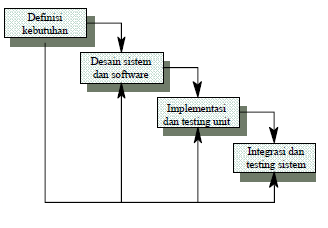
\includegraphics[width=10cm]{gambar/tahappenelitian}
    \caption{Tahapan Penelitian.}
    \label{openwrt}
\end{figure}

\section{Tempat dan Waktu Penelitian}
Tempat penelitian  dilakukan di Fakultas Teknik Informatika pada bagian PDI, waktu penelitian dilakukan selama 1 bulan yaitu pada bulan februari sampai maret 2015. Adapun yang diteliti merupakan tata cara system ujian online yang hanya dapat dilakukan melalui web browser.

\section{Studi Literatur}
Studi literatur menjelaskan dasar teori yang digunakan untuk menunjang penulisan skripsi.
Teori-teori pendukung tersebut meliputi :
\vspace{-0.5cm}
\begin{enumerate}[a.]
\begin{singlespace}
\itemsep0em
\item Web Service
\item XML
\item SOAP
\item Elearning
\end{singlespace}
\end{enumerate}

\section{Desain Sistem}
Penelitian direncanakan akan dilaksanakan selama enam bulan. Rincian rencana jadwal penelitian dicantumkan dalam tabel berikut.


\vspace{-0.5cm}
\begin{figure}[ht!]
  \centering
    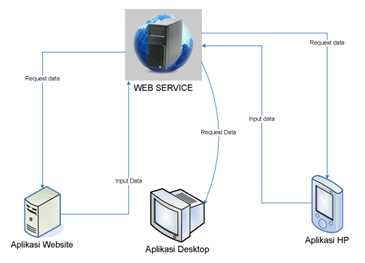
\includegraphics[width=10cm]{gambar/arsiteksistem}
    \caption{Arsitektur sistem Ujian Online.}
    \label{openwrt}
\end{figure}

\section{Analisa Dan Perancangan}
Karakteristik dan permasalahan sebuah aplikasi tanpa menggunakan Web Service :
\vspace{-0.5cm}
\begin{enumerate}[a.]
\begin{singlespace}
\itemsep0em
\item Sebuah data tidak bisa diintegrasikan dengan platform yang lain, jadi data akan stagnan di dalam satu aplikasi saja
\item Membuat aplikasi satu-satu meskipun aplikasi tersebut mempunyai fungsi yang sama, misalnya saja aplikasi web dan desktop yang memerlukan sebuah fungsi untuk melakukan fungsi kurs antar mata uang yang berbeda. Daripada membuat fungsi yang sama dua kali, lebih baik membuat kurs tersebut dalam sebuah web service.
\item Sebuah aplikasi tidak bisa diakses dari device yang berbeda
\end{singlespace}
\end{enumerate}
Dari beberapa permasalahan yang sering dihadapi pada system ujian online sendiri, maka kami ingin membuat sebuah sistem web service yang mampu memberikan solusi untuk mengintegrasikan data beda platform.
Alasan pemilihan web service sebagai solusi adalah :
\vspace{-0.5cm}
\begin{enumerate}[a.]
\begin{singlespace}
\itemsep0em
\item Sistem ujian Online yang menjadi bagian penting dalam penilaian akan lebih handal dan terstruktur jika menggunakan aplikasi client – server. Dalam hal ini Web Services yang akan bertindak sebagai server yang akan diletakkan dipusat dan aplikasi yang dimiliki oleh masing – masing  mahasiswa yang akan menjadi kliennya.
\item Web Services menggunakan protokol http sebagai komunikasi data,sehingga Ujian Online yang ingin menggunakan sistem ini tidak perlu lagi untuk membangun jaringan pribadi antara pusat dengan para mahasiswa.
\item Web Services menggunakan XML sebagai format dokumen dalam melakukan pertukaran datanya. Karena XML merupakan suatu format dokumen yang berbasis teks, maka, Web Services memungkinkan berlangsungnya komunikasi antar aplikasi yang berbeda dengan platform yang berbeda pula dan dapat menghemat waktu dalam komunikasi antara aplikasi dengan service penyedia
\end{singlespace}
\end{enumerate}

%-----------------------------------------------------------------
%Disini akhir masukan Bab
%-----------------------------------------------------------------

%-----------------------------------------------------------------
%Disini awal masukan untuk Daftar Pustaka
%-----------------------------------------------------------------
%%\nocite{Abel2010,Guerbas201350}
%%\bibliography{research-plan}
%%\bibliographystyle{plainnat}
\begin{thebibliography}{9}

\bibitem[satu(2013)]{satu01}
Chaudary, A.S, Saleem, M.A, Bukhary, H.Z. (2003). Web Services and Distributed Applications. Advantages and Problems. Internet Resources. 

\bibitem[dua(2013)]{dua02}
Endrei, M., Ang, J., Arsanjani, A., Chua, S., Comte P., Krogdahl, P., Luo, M., Newling, T. (2004). Patterns: Service-Oriented Architecture and Web Services, IBM Corp, New York.

\bibitem[tiga(2013)]{tiga03}
Freeman, A. \& Jones, A. (2003). Microsoft. NET XML Web Services Step By Step. Microsoft Press, Redmont. Washington. 

\bibitem[empat(2013)]{empat04}
Manes, Anne T. (2003). Web Services: A Manager Guide. Pearson Education Inc: Boston USA.

\bibitem[lima(2013)]{lima05}
Microsoft. (2004). Building Secure Web Services. Pattern and Practice Module. Microsoft Corporation.

\bibitem[enam(2013)]{enam06}
Microsoft. NET web site. What are XML Web Services?, URL :\url{http://www.microsoft.com/net/basics/xmlservices.asp}, diakses terakhir pada tanggal 14 Januari 2002.

\bibitem[tujuh(2013)]{tujuh07}
wikipedia web site. SOAP adalah?, URL :\url{http://id.wikipedia.org/wiki/Simple_Object_Access_Protocol}

\end{thebibliography}
\addcontentsline{toc}{chapter}{DAFTAR PUSTAKA}
%-----------------------------------------------------------------
%Disini akhir masukan Daftar Pustaka
%-----------------------------------------------------------------

\end{document}